\textbf{Chapter 4}
\[ \sum_{p\leq x}\frac{\log p}{p} \qquad \sum_{p\leq x}\frac1p \]
\textbf{Shapiro} For $a\colon\Z^+\to[0,\infty)$ if $\sum a(n)\floor{\frac xn}=x\log x+O(x)$ then $\sum a(n)\frac xn=x\log x+O(x)$
\[ \therefore \sum\frac{a(n)}n = \log x + O(1) \]
\[ \eg \qquad \sum_{n\leq x}\frac{\Lambda(n)}{n} = \log x + O(1) \]
\eg Find an asymptotic formula for $\sum_{p\leq x}\frac{\log p}{p}$ \\
\soln
\begin{align*}
\Lambda(n) &= \begin{cases}
\log p & \text{when $n=p^k$ with $p$ prime} \\
0 & \text{otherwise}
\end{cases} \\
\sum_{n\leq x}\frac{\Lambda(n)}{n} &= \sum_{p^k\leq x}\frac{\log p}{p^k} \\
&= \sum_{p\leq x}\sum_{\substack{k\geq1\\p^k\leq x}} \frac{\log p}{p^k} \\
&= \sum_{p\leq x}\paren[\Big]{\frac{\log p}{p}+\sum_{\substack{k\geq2\\p^k\leq x}}\frac{\log p}{p^k}} \\
\therefore \sum_{n\leq x}\frac{\log p}{p} &= \sum_{n\leq x}\frac{\Lambda(n)}{n} - \sum_{p\leq x}\sum_{\substack{k\geq2\\p^k\leq x}}\frac{\log p}{p^k} \\
&= \log x + O(1) + \sum_{p\leq x}\sum_{\substack{k\geq2\\p^k\leq x}}\frac{\log p}{p^k} \\
\text{\emph{and} } \sum_{p\leq x}\sum_{\substack{k\geq2\\p^k\leq x}}\frac{\log p}{p^k} &\leq \sum_{p\leq x}\sum_{k\geq2}\frac{\log p}{p^k} \\
&= \sum_{p\leq x}\log p\paren[\Big]{\frac1{p^2}+\frac1{p^3}+\frac1{p^4}+\dotsb} \\
&= \sum_{p\leq x}\frac{\log p}{p(p-1)} \\
&\leq \sum_{n=1}^\infty \frac{\log n}{n(n-1)} \text{ which converges} \\
\therefore \sum_{p\leq x}\frac{\log p}{p} &= \log x + O(1)
\end{align*}
\eg Find an asymptotic formula for $\sum_{p\leq x}\frac1p$. \\
\soln We use Abel's Summation Formula\footnote{$\sum a(n)f(n)=A(x)f(x)-\int_1^xA(t)f'(t)\d t$} with
\[ a(n) = \begin{cases}
\frac{\log p}{p} & \text{when $n=p$ is prime} \\
0 & \text{when $n$ is not prime}
\end{cases} \]
and $f(x)=\frac1{\log x}$ to get
\begin{align*}
\sum_{n\leq x}\frac1p &= \sum_{n\leq x}a(n)f(n) \\
&= A(x)f(x) - \int_1^x A(t) f'(t) \d t \\
\text{where } A(x) &= \sum_{n\leq x} a(n) \\
&= \sum_{p\leq x}\frac{\log p}{p} \\
&= \paren[\Big]{\sum_{p\leq x}\frac{\log p}{p}}\paren[\Big]{\frac{1}{\log x}} - \int_1^x \paren[\Big]{\sum_{p\leq t}\frac{\log p}{p}} \paren[\Big]{\frac{-1}{t(\log t)^2}} \d t \\
&= \paren[\Big]{\log x+O(1)} \paren[\Big]{\frac{1}{\log x}} + \int_2^x \frac{\log t+g(t)}{t(\log t)^2} \d t\footnote{note that $A(x)=0$ for $x<2$} \\
&\qquad\qquad \text{where $g(t)=\paren[\Big]{\sum_{p\leq t}\frac{\log p}{p}-\log t}=O(1)$} \\
&= 1 + O\paren[\Big]{\frac1{\log x}} + \int_2^x \frac{1}{t\log t}\d t + \int_2^x \frac{g(t)}{t(\log t)^2} \d t \\
&= 1 + O\paren[\Big]{\frac{1}{\log x}} + \brack[\Big]{\log\log t}_2^x + \int_2^\infty \frac{g(t)}{t(\log t)^2}\d t - \int_x^\infty \frac{g(t)}{t(\log t)^2}\d t \\
&= 1 + O\paren[\Big]{\frac{1}{\log x}} + \log\log x - \log\log2 + a + O\paren[\Big]{\frac{1}{\log x}}\footnote{%
since if we choose $b$ so that $\abs{g(t)}\leq b$ then
\[ \abs[\Big]{\int_x^\infty\frac{g(t)}{t(\log t)^2}\d t} \leq b\int_x^\infty\frac{\!\d t}{t(\log t)^2} = b\brack*{\frac{-1}{\log t}}_x^\infty = \frac{b}{\log x} . \]
} \\
\therefore \sum_{n\leq p}\frac{1}{p} &= \log\log x + c + O\paren[\Big]{\frac{1}{\log x}}
\end{align*}
for some constant $c$
\[ \paren[\Big]{c = 1-\log\log2+a=\lim_{x\to\infty}\paren[\Big]{\sum_{n\leq x}\frac1p-\log\log x}} \]
\eg (To motivate Dirichlet Characters) \\
Find an asymptotic formula for $\sum_{n=k\bmod l}\binom{m}{n}$ where $m$, $k$, $l\in\Z^+$. \\
\[ \soln \qquad \sum_{n\geq0}\binom{m}{n} = (1+1)^m = 2^m \footnote{Aside:
\[ \sum_{p\leq x}\frac{\log p}{p} = \log x + O(1) \qquad \sum_{\substack{p=k\bmod l\\k\in U_l}}\frac{\log p}{p} = \frac{1}{\phi(l)}\log x + O(?) \]
} . \]
Take $k=0$.  Find
\[ \sum_{n=0\bmod l}\binom{m}{n} = \binom{m}{0} + \binom{m}{l} + \binom{m}{2l} + \dotsb \]
(\ans $\sim\frac1l2^m$)

Let $\alpha=e^{i2\pi/l}$.  $C_l=\brace{1,\alpha,\alpha^2,\dotsc,\alpha^{l-1}}$, $\sum_{i=0}^{l-1}\alpha^i=0$.
\begin{align*}
(1+1)^m &= \binom{m}{0} + \binom{m}{1} + \binom{m}{2} + \dotsb \\
(1+\alpha)^m &= \binom{m}{0} + \binom{m}{1}\alpha + \binom{m}{2}\alpha^2 + \dotsb \\
(1+\alpha^2)^m &= \binom{m}{0} + \binom{m}{1}\alpha^2 + \binom{m}{2}\alpha^4 + \dotsb \\
&\eqvdots \\
(1+\alpha^{l-1})^m &= \dotsb \\
\sum_{i=1}^{l-1}(1+\alpha^i)^m &= \sum_{n=0\bmod l}l\binom{m}{n} \\
\sum_{n=0\bmod l}\binom{m}{n} &= \frac1l\sum_{i=0}^{l-1}(1+\alpha^i)^m \\
&= \frac1l\paren[\Big]{2^m+\sum_{i=1}^{l-1}(1+\alpha^i)^m}
\end{align*}
%[diagram]
\[
\myvcenter{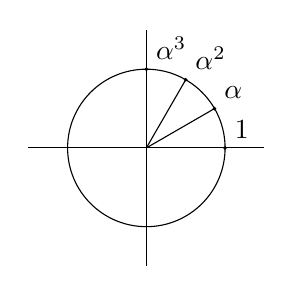
\begin{tikzpicture}
\draw(-1.5,0)--(1.5,0);
\draw(0,-1.5)--(0,1.5);
\draw(0,0)circle[radius=1];
\draw(0,0)--(30:1);
\draw(0,0)--(60:1);
\fill(0:1)circle[radius=0.025];
\fill(30:1)circle[radius=0.025];
\fill(60:1)circle[radius=0.025];
\fill(90:1)circle[radius=0.025];
\node[above right] at (0:1){$1$};
\node[above right] at (30:1){$\alpha$};
\node[above right] at (60:1){$\alpha^2$};
\node[above right] at (90:1){$\alpha^3$};
\end{tikzpicture}} \qquad\longrightarrow\qquad
\myvcenter{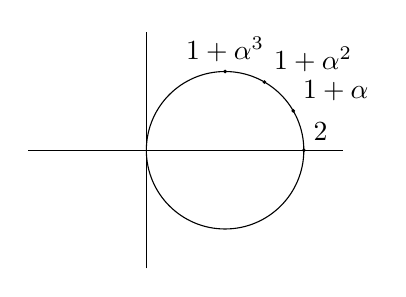
\begin{tikzpicture}
\draw(-1.5,0)--(2.5,0);
\draw(0,-1.5)--(0,1.5);
\begin{scope}[shift={(1,0)}]
\draw(0,0)circle[radius=1];
\fill(0:1)circle[radius=0.025];
\fill(30:1)circle[radius=0.025];
\fill(60:1)circle[radius=0.025];
\fill(90:1)circle[radius=0.025];
\node[above right] at (0:1){$2$};
\node[above right] at (30:1){$1+\alpha$};
\node[above right] at (60:1){$1+\alpha^2$};
\node[above] at (90:1){$1+\alpha^3$};
\end{scope}
\end{tikzpicture}}
\]
\begin{align*}
\abs[\Big]{\sum_{i=1}^{l-1}(1+\alpha^i)^m} &\leq (l-1)\abs{1+\alpha}^m \\
&= (l-1)\sqrt{\paren[\Big]{1+\cos\frac{2\pi}{l}}^2+\paren[\Big]{\sin\frac{2\pi}{l}}^2}^m \\
&= (l-1)\sqrt{2+2\cos\frac{2\pi}{l}}^m\footnote{
\begin{align*}
\cos^2\theta &= \frac{1+\cos2\theta}{2} \\
4\cos^2\theta &= 2 + 2\cos2\theta
\end{align*}} \\
&= (l-1)\paren[\Big]{2\cos\frac\pi l}^m \\
&= O\paren[\Big]{\paren[\Big]{2\cos\frac\pi l}^m} \\
\therefore \sum_{n=0\bmod l}\binom{m}{n} &= \frac1l2^m + O\paren[\Big]{\paren[\Big]{2\cos\frac\pi l}^m}
\end{align*}
To get $\sum_{n=k\bmod l}\binom{m}{n}$ find $\sum_{i=0}^{l-1}\alpha^{-ik}(1+\alpha^i)^m$.  $\alpha^{-ik}=(\overline{\alpha}^k)^i$
